\documentclass[a4paper,12pt]{article}

\usepackage{lmodern}
\usepackage[utf8]{inputenc}
\usepackage[T1]{fontenc}
\usepackage[final]{pdfpages}
\usepackage{verbatim}

\usepackage{geometry}
\geometry{
 a4paper,
 left=15mm,
 top=15mm,
}

\usepackage{xcolor}
\usepackage{listings}
% ---
% Listings
% ---
\renewcommand{\lstlistingname}{Algoritmo}% Listing -> Algoritmo
\renewcommand{\lstlistlistingname}{Lista de \lstlistingname s}% List of Listings -> Lista de Algoritmos
\definecolor{mygreen}{rgb}{0,0.6,0}
\definecolor{mygray}{rgb}{0.5,0.5,0.5}
\definecolor{mymauve}{rgb}{0.58,0,0.82}
\lstset{ %
  backgroundcolor=\color{white},     % choose the background color;
  basicstyle=\footnotesize\ttfamily, % the size of the fonts that are used for the code
  breakatwhitespace=false,           % sets if automatic breaks should only happen at whitespace
  breaklines=true,                 % sets automatic line breaking
  captionpos=t,                    % sets the caption-position to bottom
  commentstyle=\color{mygreen},    % comment style
  morecomment=[l]{//\ },           % comment only with space after //
  deletekeywords={...},            % if you want to delete keywords from the given language
  escapeinside={\%*}{*)},          % if you want to add LaTeX within your code
  extendedchars=true,              % lets you use non-ASCII characters; for 8-bits encodings only, does not work with UTF-8
  frame=single,                    % adds a frame around the code
  keepspaces=true,                 % keeps spaces in text, useful for keeping indentation of code (possibly needs columns=flexible)
  keywordstyle=\color{blue},       % keyword style
  language=[90]Fortran,                % the language of the code
  morekeywords={*,...},            % if you want to add more keywords to the set
  numbers=none,                    % where to put the line-numbers; possible values are (none, left, right)
  numbersep=5pt,                   % how far the line-numbers are from the code
  numberstyle=\tiny\color{mygray}, % the style that is used for the line-numbers
  rulecolor=\color{black},         % if not set, the frame-color may be changed on line-breaks within not-black text (e.g. comments (green here))
  showspaces=false,                % show spaces everywhere adding particular underscores; it overrides 'showstringspaces'
  showstringspaces=false,          % underline spaces within strings only
  showtabs=false,                  % show tabs within strings adding particular underscores
  stepnumber=2,                    % the step between two line-numbers. If it's 1, each line will be numbered
  stringstyle=\color{mymauve},     % string literal style
  tabsize=2,                         % sets default tabsize to 2 spaces
  title=\lstname,                  % show the filename of files included with \lstinputlisting; also try caption instead of title
  numberbychapter=false            % number lists by chapter or sequentially from the beginning of the document
}

\begin{document}


% Top matter
\title{Fortran 666 - Analisador Léxico}
\author{Makhles Reuter Lange \\ Maurilio Atila Carvalho de Santana}
\date{\today}
\maketitle

% Main document

%%%%%%%%%%%%%%%%%%%%%%%%%%%%%%%%%%%%%%%%%%%%%%%%%%%%%%%%%%%%%%%%%%%%%%%%%%%%%%
\section{Fortran 666}

O Fortran é uma linguagem de programação imperativa desenvolvida especialmente para computação numérica e científica em meados de 1950 pela IBM. Desde a sua criação, diversas versões foram desenvolvidas, dentre as quais cita-se o FORTRAN 66, o FORTRAN 77 e o Fortran 90 como as principais. A linguagem que será utilizada para a construção do compilador ao longo da disciplina utilizará características dessas diversas versões.


%%%%%%%%%%%%%%%%%%%%%%%%%%%%%%%%%%%%%%%%%%%%%%%%%%%%%%%%%%%%%%%%%%%%%%%%%%%%%%
\section{Gramática}

A gramática do Fortran 666 foi criada pelos integrantes da equipe a partir do zero. Posteriormente, consultou-se a gramática oficial do FORTRAN 77 e decidiu-se adotar alguns dos nomes dos seus símbolos não-terminais.

A descrição formal da gramática livre de contexto foi feita utilizando-se o \emph{Formalismo de Backus-Naur Estendido} (EBNF)\footnote{O EBNF é uma família de notações meta-sintaxe para a descrição formal de linguagens formais.}. A partir da gramática na forma EBNF, utilizou-se o site RailRoad\footnote{Vide http://www.bottlecaps.de/rr/ui} para gerar diagramas de sintaxe. O resultado pode ser visto na página seguinte.

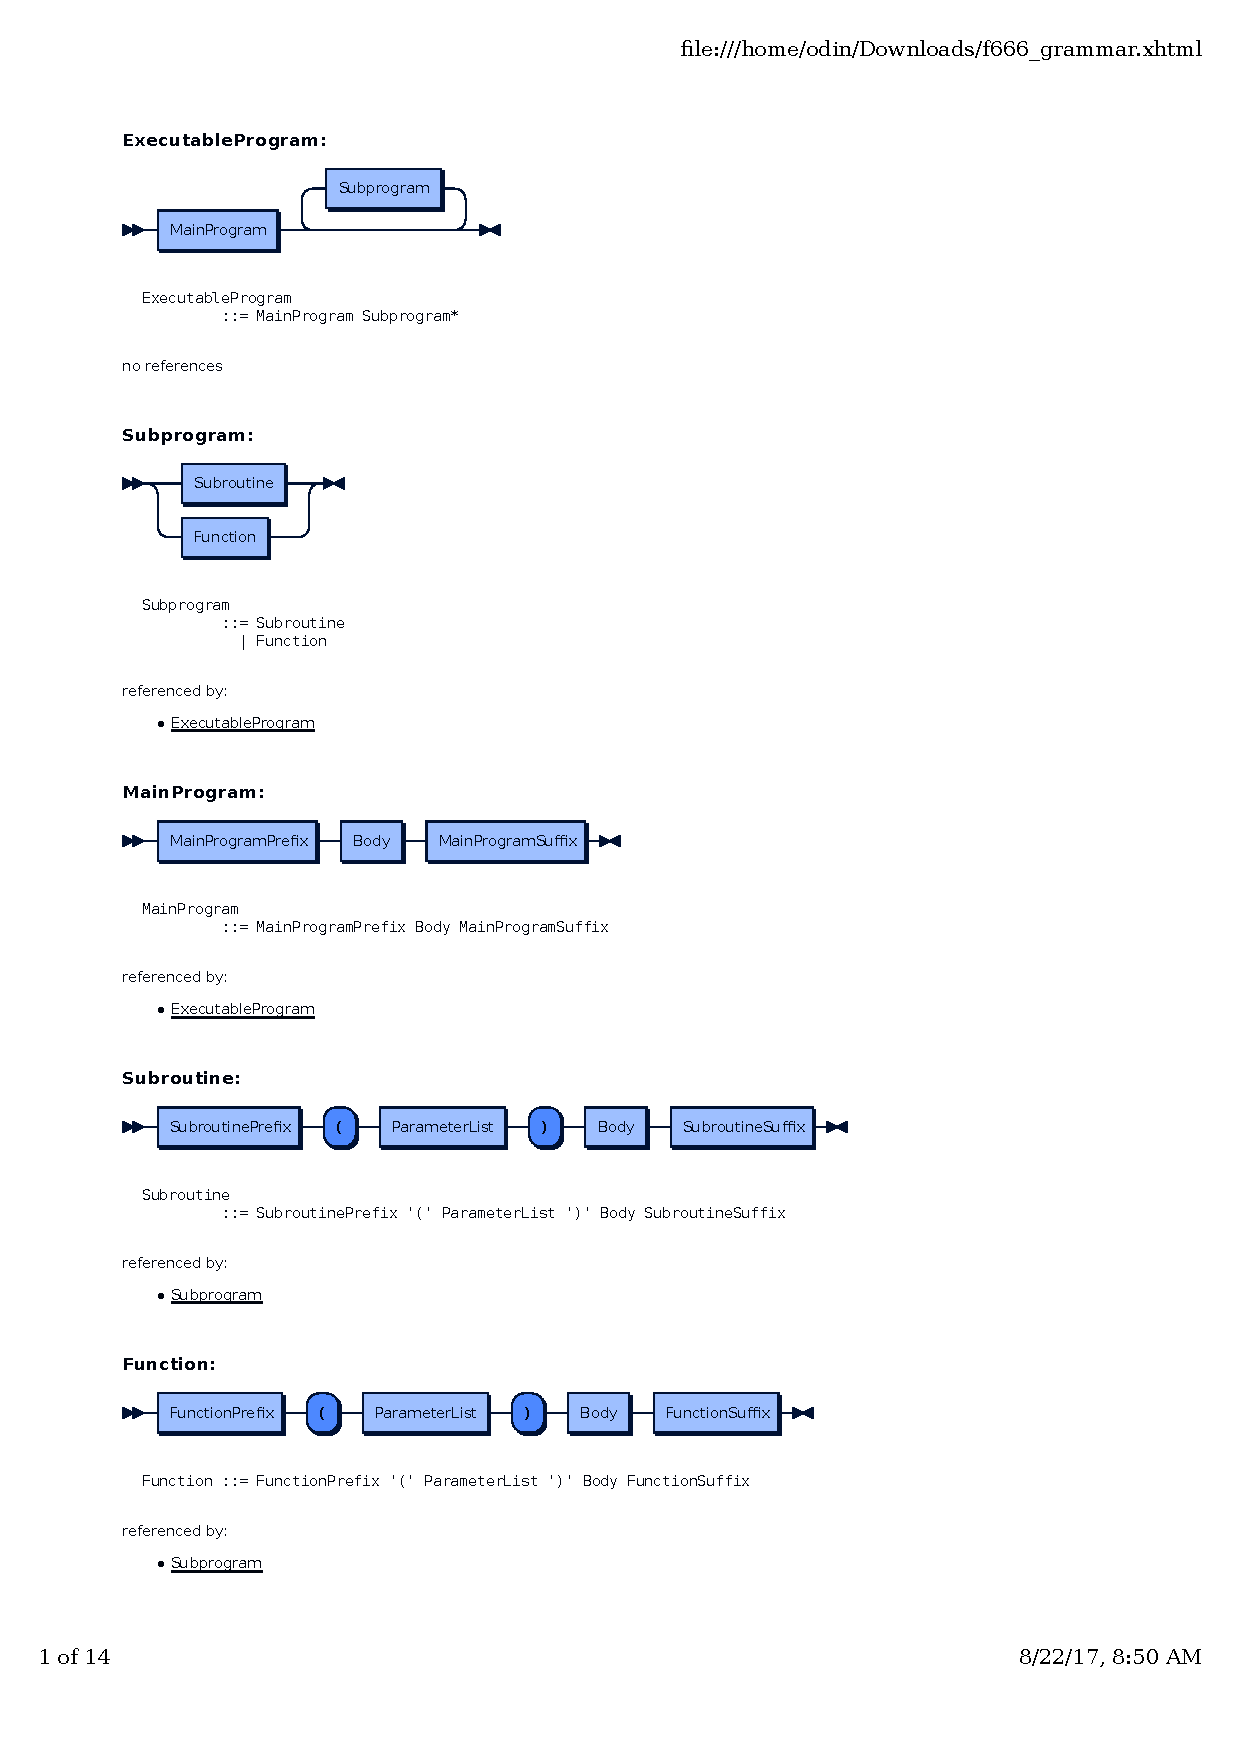
\includepdf[pages=-]{./include/fortran666_grammar.pdf}


%%%%%%%%%%%%%%%%%%%%%%%%%%%%%%%%%%%%%%%%%%%%%%%%%%%%%%%%%%%%%%%%%%%%%%%%%%%%%%
\section{Flex}

O Flex (\emph{The Fast Lexical Analyzer}) é um gerador de analisador léxico desenvolvido por Vern Paxson em 1987 sob a licença de Berkeley. Na verdade, Paxson fez apenas uma tradução para a linguagem C de uma versão do programa \emph{lex} escrita em \emph{ratfor} (um Fortran estendido), originalmente desenvolvido por Mike Lesk e Eric Schmidt em 1975.

Um programa flex consiste em três seções separadas por linhas com os símbolos \%\%. A primeira seção contém declarações e configurações; a segunda contém uma lista de padrões e ações, enquanto que a terceira contém código C que é copiado para o analisador gerado.

O arquivo flex criado, \emph{scanner.l}, pode ser visto abaixo. 

\verbatiminput{../scanner.l}


%%%%%%%%%%%%%%%%%%%%%%%%%%%%%%%%%%%%%%%%%%%%%%%%%%%%%%%%%%%%%%%%%%%%%%%%%%%%%%
\section{Geração do analisador léxico}

Ao rodar o programa flex passando-se o arquivo \emph{scanner.l}, cria-se a rotina de análise léxica em C: \emph{lex.yy.c}. Esse program deve ser compilado fazendo-se a ligação com a biblioteca \texttt{lbl}:

\begin{verbatim}
$ flex scanner.l
$ gcc lex.yy.c -lbl -o scanner
\end{verbatim}
%
O analisador léxico gerado (\emph{scanner}) encontra-se junto aos arquivos compactados.


%%%%%%%%%%%%%%%%%%%%%%%%%%%%%%%%%%%%%%%%%%%%%%%%%%%%%%%%%%%%%%%%%%%%%%%%%%%%%%
\section{Programas-teste}

Para testar a identificação dos \emph{tokens}, criou-se quatro arquivos escritos em Fortran 666, listados a seguir.

\lstinputlisting[frame=single]{../test/swap.f}
\lstinputlisting[frame=single]{../test/rain.f}
\lstinputlisting[frame=single]{../test/matmul.f}
\lstinputlisting[frame=single]{../test/error.f}


%%%%%%%%%%%%%%%%%%%%%%%%%%%%%%%%%%%%%%%%%%%%%%%%%%%%%%%%%%%%%%%%%%%%%%%%%%%%%%
\section{Identificação dos \emph{tokens}}

A identificação dos \emph{tokens} foi feita passando-se cada um dos arquivos listados no item anterior para o analisador léxico gerado, \emph{scanner}. A impressão dos \emph{tokens} é feita no próprio console.

Para facilitar a sua identificação, ao invés de imprimir cada \emph{token} em uma linha separada, os \emph{tokens} foram impressos nas mesmas linhas em que se encontravam no respectivo arquivo fonte. Os resultados obtidos se encontram nos arquivos com extensão \texttt{.stream} e podem ser vistos a seguir.

\begin{verbatim}
$ ./scanner ./test/swap.f
\end{verbatim}
\lstinputlisting[frame=single]{../test/swap.stream}

\begin{verbatim}
$ ./scanner ./test/rain.f
\end{verbatim}
\lstinputlisting[frame=single]{../test/rain.stream}

\begin{verbatim}
$ ./scanner ./test/matmul.f
\end{verbatim}
\lstinputlisting[frame=single]{../test/matmul.stream}

\begin{verbatim}
$ ./scanner ./test/error.f
\end{verbatim}
\lstinputlisting[frame=single]{../test/error.stream}


\end{document}